\documentclass[12pt, oneside]{article}
\usepackage[utf8]{inputenc}
\usepackage{polski}
\renewcommand*{\figurename}{Rys.}
\usepackage{graphicx}
\usepackage{float}
\usepackage{geometry}
\usepackage{subcaption}
\usepackage{indentfirst}
\geometry{
	left=25mm,
	right=25mm,%
	bindingoffset=10mm, 
	top=25mm, 
	bottom=25mm}
\title{
	Eksploracyjna analiza danych \\
	Światowy program szczepień przeciwko COVID-19
}
\author{
	Marek Grudkowski 156587
	\\
	Kamil Kaczmarkiewicz 171701
}

\begin{document}

\maketitle

\section{Ogólny opis danych}

Zbiór danych dotyczy aktualnego postępu poszczególnych państw w szczepieniach przeciwko COVID-19. Zawiera on informacje pochodzące prawie ze wszystkich krajów na świecie podzielone na poszczególne dni. Program szczepień przeciwko COVID to w dobie pandemii niezwykle gorący temat. Naszym zdaniem warto się na nim skupić, gdyż może zawierać wiele ukrytych informacji, które mogą przydać się w walce z pandemią i przyspieszyć sam proces szczepień. 

\section{Cel eksploracji i kryteria sukcesu}

Celem eksploracji danych jest zgłębienie wszelkich tajemnic ukrytych w analizowanym zbiorze danych. Takie informacje można wykorzystać do wskazania zarówno państw, które najlepiej przeprowadzają program szczepień, jak i tych w których proces ten przebiega bardzo słabo. Dzięki temu niektóre państwa mogłyby się wzorować na tych państwach, które radzą sobie najlepiej oraz uniknąć błędów, jakie popełniły najgorsze w rankingu państwa.  Dodatkowym celem może być predykcja zapotrzebowania szczepionek w danych krajach na najbliższe miesiące, która mogłaby by zapobiec marnowaniu się dawek oraz pozwolić rządom na świecie lepiej zaplanować \textit{zakupy} oraz logistykę akcji na terenie swoich państw.  Jako ostatni cel można uznać wskazanie prawdopodobnej daty zakończenia światowego programu szczepień. 
\par
Jako kryteria sukcesu eksploracji danych można uznać odpowiednio wysoką (przykładowo $80$ \%) zgodność predykcji wykonywanych szczepień w danych państwach z rzeczywistymi danymi, które są aktualizowane na bieżąco. 

\newpage

\section{Charakterystyka zbioru danych}
Zbiór danych na stan dnia pisania tego sprawozdania zawiera ponad 13300 przykładów. Dane aktualizowane są zazwyczaj co kilka dni i pochodzą z wielu różnych źródeł. Zazwyczaj są nimi organy krajowe lub lokalne, czy międzynarodowe organizacje. Dla każdego przykładu podane jest źródło i jego adres internetowy, co daje możliwość weryfikacji w przypadku jakichkolwiek wątpliwości co do poprawności danych. Dane zapisane są w jednym pliku w formacie csv i podzielone są na następujące kolumny:

\paragraph{country}
\mbox{}\\
Nazwa państwa lub regionu, którego dotyczy dany przykład.

\paragraph{ISO code}
\mbox{}\\
Trzyliterowy kod państwa zgodny z normą ISO $3166-1$

\paragraph{date}
\mbox{}\\
Data pozyskania danych. 

\paragraph{total vaccinations}
\mbox{}\\
Całkowita liczba podanych dawek. Zliczane są tutaj pojedyncze dawki i nie mogą być równe całkowitej liczbie zaszczepionych osób, w zależności od schematu dawkowania np. jedna osoba może przyjąć kilka dawek.

\paragraph{total vaccinations per hundred}
\mbox{}\\
Całkowita liczba podanych dawek szczepionki w przeliczeniu na sto osób w liczbie ludności całego kraju.

\paragraph{daily vaccinations raw}
\mbox{}\\
Dzienna zmiana w całkowitej liczbie podanych dawek. Oblicza się ją tylko dla kolejnych dni. Surowy środek w celu kontroli danych i jej przejrzystości. Autorzy zestawu nie zalecają korzystania z tego atrybutu. 

\paragraph{daily vaccinations}
\mbox{}\\
Liczba dawek podawanych dziennie. Liczba ta jest wygładzana w ujęciu 7 dni. W przypadku krajów, które nie przekazują danych w ujęciu dziennym zakłada się, że dawki zmieniały się jednakowo we wszystkich okresach, w których nie przekazywano danych. Tak wypełnione dane uśrednia się dodatkowo w 7 dniowym oknie.

\paragraph{daily vaccinations per million}
\mbox{}\\
Liczba dawek podawanych dziennie w przeliczeniu na milion osób w ludności całego kraju

\paragraph{people vaccinated}
\mbox{}\\
Całkowita liczba osób, które otrzymały przynajmniej jedną dawkę szczepionki. Jeśli osoba otrzyma pierwszą dawkę liczba zwiększana jest jeden, jeśli otrzyma drugą, pozostaje taka sama. 

\paragraph{people vaccinated per hundred}
\mbox{}\\
Całkowita liczba osób, które otrzymały przynajmniej jedną dawkę szczepionki w przeliczeniu na sto osób w liczbie ludności całego kraju.

\paragraph{people fully vaccinated}
\mbox{}\\
Całkowita liczba osób, które otrzymały wszystkie dawki zgodnie ze schematem szczepienia. Jeśli bierzemy pod waugę schemat szczepień z dwoma dawkami - przy pierwszej dawce liczba nie zmienia się, po drugiej dawce zwiększana jest o 1. 

\paragraph{people fully vaccinated per hundred}
\mbox{}\\
Całkowita liczba osób, które otrzymały wszystkie dawki zgodnie ze schematem szczepienia w przeliczeniu na sto osób w liczbie ludności całego kraju.

\paragraph{source name}
\mbox{}\\
Nazwa źródła, z którego pochodzą dane.

\paragraph{source website}
\mbox{}\\
Strona internetowa, źródła z którego pochodzą dane. 



\section{Eksploracyjna analiza danych}


\subsection{Atrybuty nominalne}

Podczas \textit{stricte} pracy z danymi część atrybutów będzie nieprzydatna. Do takich atrybutów z pewnością należy źródło danych oraz jego adres w Internecie. Z tego powodu można pozbyć się tych kolumn i zmniejszyć rozmiar naszego zbioru.

Kolejny brany pod uwagę atrybut, który jest do odrzucenia to kod państwa. Przy wizualizacji wyników nie powie on dużo osobie, gdyż są to tylko 3 litery. Może jednak okazać się on przydatny w walidacji innego atrybutu jakim jest państwo. Zgodnie z opisem zbioru dostarczonym przez jego autorów część przykładów nie opisuje państw, lecz regiony wchodzące w skład innych państw np. Szkocja. Znając długość kodów ISO dla państw można wyodrębnić te przykłady, które dotyczą regionów:
\begin{verbatim}
England has code OWID_ENG
Kosovo has code OWID_KOS
Northern Cyprus has code OWID_CYN
Northern Ireland has code OWID_NIR
Scotland has code OWID_SCT
Wales has code OWID_WLS
\end{verbatim}

Na początku został poprawiony kod przykładów, które dotyczą Kosowa. Kod wg normy ISO powinien mieć postać \textit{XKX} i na taki został zmieniony. Kolejnym krokiem było wcielenie przykładów dotyczących Północnego Cypru do Cypru. W tym przypadku zmiana dotyczyła zarówno kolumny \textit{country}, jak i \textit{iso\_code}. Anglia, Walia, Irlandia Północna oraz Walia są regionami, które wchodzą w skład Wielkiej Brytanii. Poprawnym rozwiązaniem w ich przypadku takich przykładów będzie dołączenie nich do Wielkiej Brytanii.

\subsection{Atrybuty numeryczne}

Pierwszym krokiem w analizie atrybutów numerycznych jest sprawdzenie, w jakiej liczbie występują braki w każdej kolumnie. Wyniki operacji sprawdzającej ten fakt, poniżej:

\begin{verbatim}
Size of data is: (13307, 13)
Missing values in dataset: 
country                                   0
iso_code                                  0
date                                      0
total_vaccinations                     5255
people_vaccinated                      5931
people_fully_vaccinated                7926
daily_vaccinations_raw                 6529
daily_vaccinations                      220
total_vaccinations_per_hundred         5255
people_vaccinated_per_hundred          5931
people_fully_vaccinated_per_hundred    7926
daily_vaccinations_per_million          220
vaccines                                  0
\end{verbatim}

Niestety jest są to bardzo duże braki, którymi należało się zająć. Na pierwszy rzut oka widać, że atrybuty łączą się w pary pod dwoma względami: nazwą oraz liczbą brakujących wartości. Zgodnie z opisem danych dostarczonym przez autorów w takiej jeden z atrybutów jest zależny od drugiego i pokazuje daną wartość w stosunku do populacji danego kraju. Aby upewnić się można sporządzić wykres prezentujący wartość korelacji pomiędzy poszczególnymi atrybutami (Rysunek \ref{Rys:cor})

\begin{figure}[h]
\centering
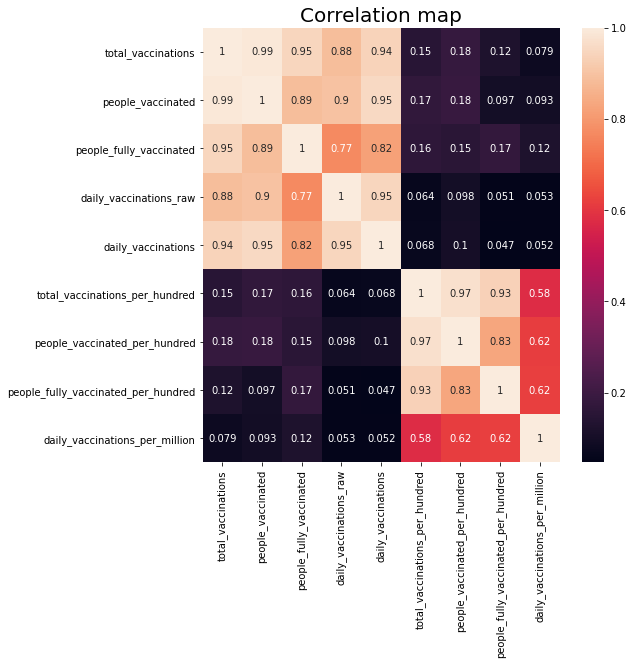
\includegraphics[width=0.8\textwidth]{../img/corelation.png} 
\caption{Korelacja pomiędzy atrybutami całego zbioru danych\label{Rys:cor}}

\end{figure}

Nie widać tutaj zależności o których wspomnieli autorzy. Powodem tego jest liczenie korelacji dla całego zbioru danych, a nie dla konkretnego państwa. Jeśli do funkcji rysującej wykres przekażemy tylko zakres danych obejmujący jedno państwo totalnie zmienia on swój wygląd. Przykładowy wykres dla Stanów Zjednoczonych można zobaczyć na rysunku nr \ref{Rys:usa}.

\begin{figure}[h]
\centering
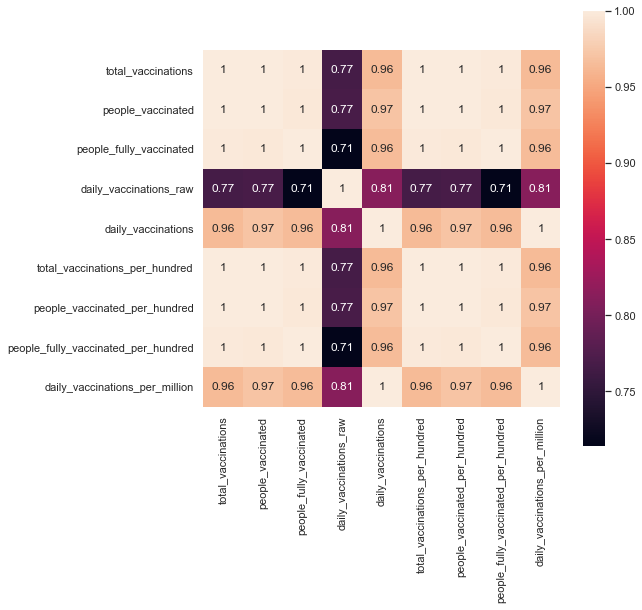
\includegraphics[width=0.8\textwidth]{../img/usa_corr.png} 
\caption{Korelacja pomiędzy atrybutami zbioru danych dla USA}
\label{Rys:usa}
\end{figure}

Aby upewnić się, czy dla wszystkich państw występuje opisana zależność, można osobno dla każdego państwa obliczyć korelację pomiędzy atrybutami i sporządzić histogram, na którym role pojedynczych próbek będą pełnić państwa (Rysunek \ref{Rys:hist}). Zdecydowanie widać, że na każdym z owych wykresów niemal 100\% próbek wskazywało na korelację równą 1, co oznacza zgodność z tym, co napisali autorzy zestawu danych.

\begin{figure}
  \begin{subfigure}[t]{.45\textwidth}
    \centering
    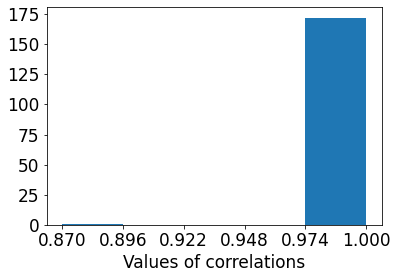
\includegraphics[width=\linewidth]{../img/null_column_diff1.png}
    \caption{Korelacja między dzienną liczbą wykonanych szczepień ogółem i na milion osób}
  \end{subfigure}
  \hfill
  \begin{subfigure}[t]{.45\textwidth}
    \centering
    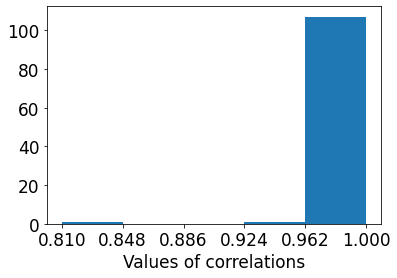
\includegraphics[width=\linewidth]{../img/null_column_diff2.png}
    \caption{Korelacja między liczbą ludzi w pełni zaszczepionymi ogółem i na 100 osób}
  \end{subfigure}

  \medskip

  \begin{subfigure}[t]{.45\textwidth}
    \centering
    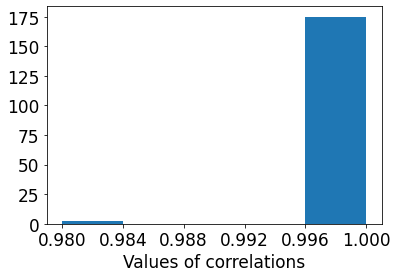
\includegraphics[width=\linewidth]{../img/null_column_diff3.png}
    \caption{Korelacja między liczbą ludzi którzy przyjęli choć jedną dawkę ogółem i na 100 osób}
  \end{subfigure}
  \hfill
  \begin{subfigure}[t]{.45\textwidth}
    \centering
    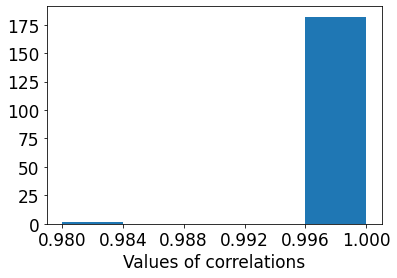
\includegraphics[width=\linewidth]{../img/null_column_diff4.png}
    \caption{Korelacja między liczbą wykonanych szczepień ogółem i na sto osób}
  \end{subfigure}
  \caption{Korelacje pomiędzy poszczególnym atrybutami zbioru}
\label{Rys:hist}
\end{figure}

Jedynym atrybutem który pozostał bez pary jest \textit{daily\_vaccinations\_raw}. Jednakże wedle zaleczeń autorów zestawu nie powinien być uwzględniany podczas analizy, dlatego można z niego zrezygnować. 

Pierwszym atrybutem, w którym łatwo można uzupełnić dane jest \textit{total\_vaccinations}. Dotyczy on łącznej sumy wykonanych szczepień w danym państwie. W przypadku brakujących wartości można je wypełnić zakładając idealną liniową progresję pomiędzy odległymi wartościami.

Po wypełnieniu kolumny z totalną liczbą podanych dawek, można łatwo uzupełnić kolumnę opisującą średnią liczbę podanych dawek na sto osób. Wystarczy dla brakujących wartości wstawić liczbę opisaną zależnością:
\begin{verbatim}
liczbaPodanychDawekNaSto = totalnaLiczbaPodanychDawek / ludnoscKraju * 100 
\end{verbatim}

Aby to zrobić najpierw potrzebna jest liczba ludności w danym kraju. Aby wykorzystać w pełni nasz zbiór danych wielkość tą obliczyliśmy dla każdego państwa na podstawie średniego ilorazu liczby podanych dawek oraz liczby podanych dawek na sto osób, przy czym tutaj braliśmy pod uwagę tylko przykłady, w których nie brakowało żadnych wartości. Ostatecznie po wypełnieniu tych atrybutów liczba brakujących danych wygląda następująco:
\begin{verbatim}
country                                   0
iso_code                                  0
date                                      0
total_vaccinations                        0
people_vaccinated                      6069
people_fully_vaccinated                8069
daily_vaccinations                      226
total_vaccinations_per_hundred            0
people_vaccinated_per_hundred          6069
people_fully_vaccinated_per_hundred    8069
daily_vaccinations_per_million          226
vaccines                                  0
\end{verbatim}


\begin{itemize}
\item mechanizm daily vacc
\item wypełnienie luk w daily vacc
\item wykresy pudełkowe
\item podsumowanie
\end{itemize}












\end{document}
